\section{Primary Chilled Water Loop -- Chiller(s) and purchased cooling}\label{primary-chilled-water-loop-chillers-and-purchased-cooling}

The Secondary Cooling system is constructed by using a \emph{PlantLoop} object. It uses two chillers (a small constant COP chiller and a bigger electric chiller) and purchased district cooling. Therefore, the supply side of the loop contains the chillers and the purchased cooling, and the demand side contains one side of the plate heat exchanger. The loop is operated by using plant equipment operation schemes and schedules. Refer to Figure~\ref{fig:simple-line-diagram-for-the-primary-chilled} for a simple diagram of the Primary Cooling Loop.

\begin{figure}[hbtp] % fig 90
\centering
\includegraphics[width=0.9\textwidth, height=0.9\textheight, keepaspectratio=true]{media/image090.png}
\caption{Simple line diagram for the primary chilled water loop \protect \label{fig:simple-line-diagram-for-the-primary-chilled}}
\end{figure}

\subsection{Flowcharts for the Primary Chilled Water Loop Input Process}\label{flowcharts-for-the-primary-chilled-water-loop-input-process}

This series of flowcharts serve as a guide for identifying and inputting the Primary Chilled Water loop and its components into the input file. The working fluid in this loop is water. The EnergyPlus line diagram for this loop is provided in Figure~\ref{fig:energyplus-line-diagram-for-the-primary}. A simple flowchart for the separation of the half loops is provided in Figure~\ref{fig:simple-flowchart-for-the-separation-of-half}.

\begin{figure}[hbtp] % fig 91
\centering
\includegraphics[width=0.9\textwidth, height=0.9\textheight, keepaspectratio=true]{media/image091.png}
\caption{EnergyPlus line diagram for the primary chilled water loop \protect \label{fig:energyplus-line-diagram-for-the-primary}}
\end{figure}

\begin{figure}[hbtp] % fig 92
\centering
\includegraphics[width=0.9\textwidth, height=0.9\textheight, keepaspectratio=true]{media/image092.png}
\caption{Simple flowchart for the separation of half-loops in the primary chilled water loop \protect \label{fig:simple-flowchart-for-the-separation-of-half}}
\end{figure}

\subsubsection{Primary Cooling System Supply Side Loop Construction}\label{primary-cooling-system-supply-side-loop-construction}

The main components on the supply side half loop for the primary chilled water loop are two chillers and district cooling object that supply chilled water and the constant speed pump that circulates the chilled water through the loop. This pump (`CW Primary Circ Pump') is the primary pump in the primary/secondary pumping setup. This half loop supplies chilled water to the plate heat exchanger which is placed on the demand side half loop. The supply side half loop contains six components, six branches, twelve nodes, and one splitter-mixer pair. The EnergyPlus line diagram for the Primary Cooling loop supply side is provided in Figure~\ref{fig:energyplus-line-diagram-for-the-supply-side-005}. The flowchart for supply side branches and components is provided in Figure 94. The flowchart for supply side connectors is provided in Figure 95.

\begin{figure}[hbtp] % fig 93
\centering
\includegraphics[width=0.9\textwidth, height=0.9\textheight, keepaspectratio=true]{media/image093.png}
\caption{EnergyPlus line diagram for the supply side of the primary chilled water loop \protect \label{fig:energyplus-line-diagram-for-the-supply-side-005}}
\end{figure}

\begin{figure}[htbp]
\centering
\includegraphics{media/image094.png}
\caption{}
\end{figure}

Figure 94 -- Flowchart for Primary Cooling Loop supply side branches and components

\begin{figure}[htbp]
\centering
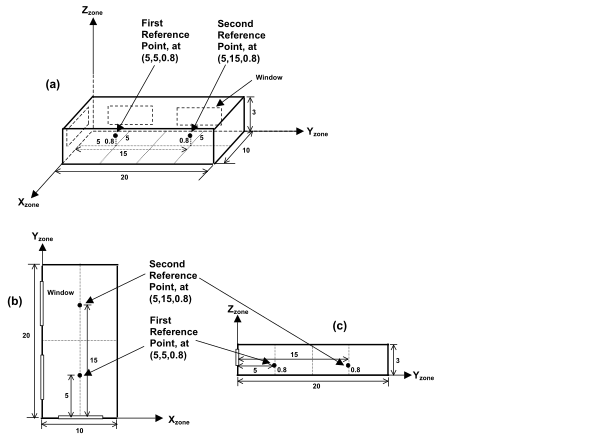
\includegraphics{media/image095.png}
\caption{}
\end{figure}

Figure 95 -- Flowchart for Primary Cooling Loop supply side connectors

\subsubsection{Primary Cooling Loop Demand Side Loop Construction}\label{primary-cooling-loop-demand-side-loop-construction}

The main component on the demand side half loop is the plate heat exchanger that facilitates the exchange of heat between the fluids of the primary and secondary chilled water loop. The plate heat exchanger will not be discussed in this loop. Instead the object will be discussed in the supply side half loop of the secondary chilled water loop. This side of the loop also has eight nodes, four components, four branches, and one splitter mixer pair. An EnergyPlus schematic for the demand side is provided in Figure 96. The flowchart for demand side branch definition is provided in Figure 97. The flowchart for the demand side connectors is provided in Figure 98.

\textbf{
\includegraphics{media/image096.png}}

Figure 96 - EnergyPlus line diagram for the demand side of the primary chilled water loop

\begin{figure}[htbp]
\centering

\includegraphics{media/image097.png}
\caption{}
\end{figure}

Figure 97 -- Flowchart for primary chilled water loop demand side branches and components

\begin{figure}[htbp]
\centering
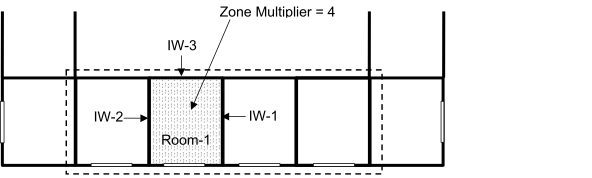
\includegraphics{media/image098.png}
\caption{}
\end{figure}

Figure 98 -- Flowchart for primary chilled water loop demand side connectors

\subsection{Flowcharts for Primary Chilled Water Loop Controls}\label{flowcharts-for-primary-chilled-water-loop-controls}

The Primary Cooling loop is operated by using set-points, plant equipment operation schemes and schedules. The plant equipment scheme for the on peak and off peak operation of the chillers is very important

\subsubsection{Primary Chilled Water Loop Schedules}\label{primary-chilled-water-loop-schedules}

The Primary Cooling loop uses three different schedules to operate properly. \emph{On Peak} is a compact schedule that defines the on peak hours (9 AM to 6 PM). The \emph{Off Peak} is a compact schedule that defines the off peak hours (6 PM to 9 AM). This plant loop also uses another compact schedule named \emph{CW Loop Temp Schedule} declare that the temperature of the chilled water loop outlet flow is 6.7 degrees Celsius at all times. This schedule is used by the setpoint manager (\emph{Primary CW Loop Setpoint Manager)}. This schedule uses a schedule type limit named \emph{Temperature,} which defines the loop upper and lower temperature limits. The flowchart for Primary Cooling loop schedule definition is provided in Figure 99.

\begin{figure}[htbp]
\centering
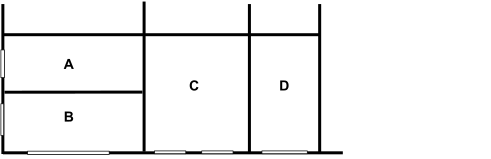
\includegraphics{media/image099.png}
\caption{}
\end{figure}

Figure 99 -- Flowchart for primary chilled water loop schedules

\subsubsection{Primary Chilled Water Loop Plant Equipment Operation Schemes}\label{primary-chilled-water-loop-plant-equipment-operation-schemes}

There are two important operation schemes in the primary chilled water loop. The \emph{CW Loop Operation} plant equipment operation scheme used two schedules (\emph{On Peak} and \emph{off Peak}) to control the supply components in the primary cooling loop. \emph{Peak Operation} is set up such that different components or combinations of components are operated for different values of cooling load during the peak hours (9AM to 6PM everyday) of the simulation period. Up to 25,000 W of cooling load, the small constant COP chiller is operated, for 25,000-245,000 W the big electric chiller and purchased cooling are used and for 245,000-500,000 W purchased cooling is used. This setup serves to increase the efficiency of the system. \emph{Off Peak Operation} is set up such that both the chillers are operated during the off peak hours (6 PM to 9 AM). Flowcharts detailing the chilled water loop plant equipment operation schemes are provided in Figure 100 and Figure~\ref{fig:flowchart-for-off-peak-plant-operation-of}.

\begin{figure}[htbp]
\centering
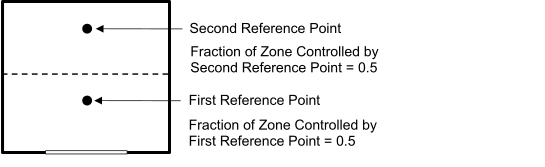
\includegraphics{media/image100.png}
\caption{}
\end{figure}

Figure 100 -- Flowchart for on peak operation of the primary chilled water loop

\begin{figure}[hbtp] % fig 101
\centering

\includegraphics[width=0.9\textwidth, height=0.9\textheight, keepaspectratio=true]{media/image101.png}
\caption{Flowchart for off peak plant operation of the primary chilled water loop \protect \label{fig:flowchart-for-off-peak-plant-operation-of}}
\end{figure}

\subsubsection{Primary Chilled Water Loop Setpoints}\label{primary-chilled-water-loop-setpoints}

The \emph{Primary CW Loop Setpoint Manager} uses the \emph{CW Loop Temp Schedule} to set a temperature control point at the \emph{CW Primary Supply Outlet Node}. This setpoint allows the program to control the temperature at the node by operating the components in the Primary Cooling loop. ~Since, setpoint managers are high-level control objects, their usefulness is realized in much more complex systems, where multiple nodes have to be monitored in order to operate the system properly. A flowchart for Secondary Cooling loop setpoints is provided in Figure 102.

\begin{figure}[htbp]
\centering
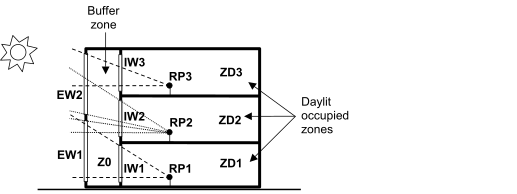
\includegraphics{media/image102.png}
\caption{}
\end{figure}

Figure 102 -- Flowchart for Primary Cooling Loop setpoints
